\section{Stalag Might}\label{stalag-might}


\begin{figure}
\centering
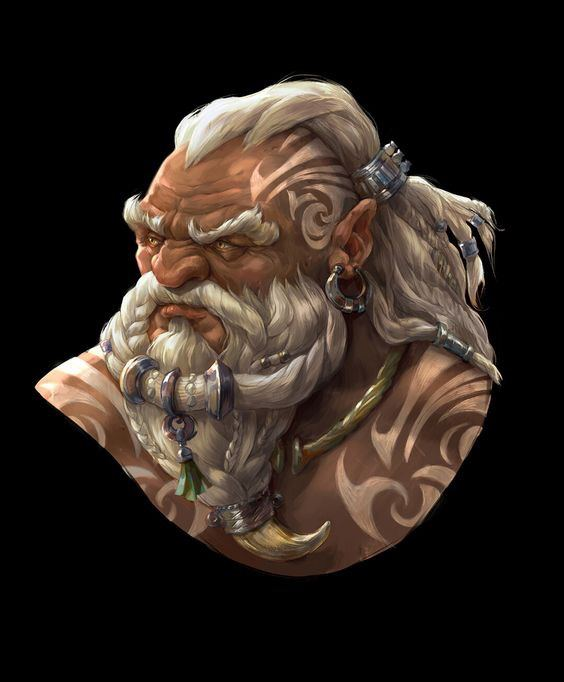
\includegraphics{2023-09-17_22.34.48.jpg}
\caption{2023-09-22.34.48.jpg}
\end{figure}

Informazioni Generali

Età:

Data di nascita:

Luogo di nascita: Lunacrest

Razza: Nano

Classe: Druido

Alleati:

Nemesi:

Alias:

Professione: Il bambino delle rocce


\subsection{Descrizione Generale}\label{descrizione-generale}


Stalag Might è un nano druido le cui origini sono radicate nelle
profondità di una montagna antica conosciuta come ``Lunacrest''. La sua
storia è intrecciata con il mistero di questa montagna, dove le energie
dell'antica luna scorrono nelle vene stesse della terra. Conosciuto tra
i druidi come il ``Bambino delle Rocce'', Stalag ha sempre mostrato una
connessione innata con le pietre e una passione per la geologia.

\begin{quote}
``Bella questa roccia''
\end{quote}

\subsection{Biografia}\label{biografia}


\subsubsection{Infanzia}\label{infanzia}


Stalag Might nacque nelle viscere di Lunacrest, portando con sé una
strana formazione rocciosa sulla mano sinistra, simile alle maestose
montagne circostanti. Questo segno innato attirò l'attenzione dei suoi
genitori, che lo condussero alla congrega dei druidi del Circolo della
Luna quando era ancora un neonato. Il giovane nano cresceva, diventando
noto tra i druidi come il ``Bambino delle Rocce''. La sua forza fisica e
la sua passione per la geologia lo resero un apprendista straordinario.

\subsubsection{Adolescenza}\label{adolescenza}


Durante gli anni della sua formazione, Stalag sviluppò un profondo
interesse per la metamorfosi, una delle abilità centrali dei druidi del
Circolo della Luna. A differenza dei suoi compagni, prediligeva
trasformarsi in piccoli animali, come topi, talpe e lucertole, per
esplorare fessure e cavità inaccessibili. Questa abilità gli consentiva
di scoprire gemme nascoste e segreti geologici, e raccontava avventure
vissute attraverso gli occhi di un piccolo animale.

\subsubsection{Età Adulta}\label{etuxe0-adulta}


Durnan Crystalbeard, il suo anziano maestro druido, riconoscendo il
talento e la dedizione di Stalag, gli regalò un geode speciale quando il
giovane nano compì sedici anni. Questo geode, inciso con simboli
druidici, divenne sia un focus per la sua magia che un santuario per
campioni di rocce e minerali rari. Dopo aver completato la sua
formazione con la congrega, Stalag sentì il richiamo dell'esplorazione e
del desiderio di scoprire montagne e formazioni rocciose leggendarie,
alla ricerca in particolare della pietra leggendaria nota come ``Il
Cuore della Luna''.

\subsection{Personalità}\label{personalituxe0}


Stalag Might è noto per la sua mente curiosa e la passione incrollabile
per la geologia. È un individuo tranquillo ma osservatore, sempre
desideroso di ascoltare le storie delle pietre e dei minerali che
incontra lungo il suo cammino. La sua connessione con la natura e il
mondo sotterraneo lo rende rispettoso nei confronti dell'ambiente
circostante.

Inoltre, la sua abilità unica di trasformarsi in creature più piccole
gli conferisce una prospettiva unica sulla vita e sull'esplorazione.
Stalag è affezionato ai suoi compagni druidi e considera ogni avventura
come un'opportunità per arricchire la sua comprensione delle meraviglie
naturali del mondo.

Stalag Might è guidato da una doppia missione: la sete di conoscenza
geologica e la ricerca dell'enigmatica ``Pietra della Luna''. Questo
equilibrio tra scienza e magia guida le sue azioni mentre viaggia
attraverso il mondo, pronta a esplorare e a svelare i segreti che
attendono sotto le rocce e nelle profondità della terra.

\subsection{Coinvolgimenti in Eventi
Recenti}\label{coinvolgimenti-in-eventi-recenti}


\href{Untitled\%20Database\%20da6a05127a584f75a0bd57df6960b00a.csv}{Untitled
Database}

